\chapter{Implementación del sistema} \label{cap:capitulo6}

\section{Metodología de trabajo}

Para el desarrollo del proyecto, al menos en la parte relativa a la implementación, se ha escogido una metodología de trabajo ágil que permita cambios de todo tipo durante todo su ciclo de vida. Esto resulta necesario debido a la naturaleza del proyecto, ya que por una parte, aunque el objetivo del proyecto es claro (desarrollar un software capaz de controlar el nivel de ruido de un local), las tareas para conseguirlo no lo son tanto, y se asume que irán  evolucionando y cambiando lo largo del proyecto. Por otro lado, la total inexperiencia en el campo de la acústica y la electrónica suponen un riesgo añadido.

Desde el comienzo del proyecto se han realizado cada martes en el laboratorio de \glsname{granasat} \textbf{reuniones semanales} en las que participan todos los miembros involucrados en el desarrollo del proyecto de alguna u otra manera, esto es, las personas nombradas en la sección \ref{sec:team} al comienzo de este documento. Las veces que no se han podido realizar de forma presencial debido a la situación actual de pandemia causada al Covid-19, se han realizado de forma remota mediante videoconferencias.

Aunque la metodología seguida no se corresponde fielmente a la metodología \textit{SCRUM}, sí que se asemeja en muchos aspectos. Si hacemos la correspondencia, \myProf\ asume, por una parte, el rol de \textit{Product Owner}, ya que entabla comunicación directa con el cliente, y por otra el rol de \textit{Scrum Master}, ya que ha sido el supervisor de todo el trabajo realizado y ha tomado las decisiones técnicas de más alto nivel. El resto de los participantes asumiríamos el rol del \textit{Equipo de desarrollo}.

La etapa de implementación se ha planificado con una duración de 5 semanas, sin ningún tipo de restricción o limitación dentro de ellas (sin \textit{sprints}). La implementación se ha realizado de forma incremental y en bloque, desarrollando el backend, la \glsname{API-REST} y pruebas conforme se iba avanzando en el desarrollo.

\section{Herramientas utilizadas}

En la tabla \ref{tab:presupuesto-software} se presentan una lista con el software utilizado durante el proyecto.

\begin{itemize}
	\item Para leer y desarrollar código se ha utilizado el \acrshort{IDE} de Microsoft: Visual Studio Code, mientras que para el control de versiones y se ha utilizado Git.

	\item Para la generación de diagramas se ha usado Visual Paradigm e Inkscape.

	\item OpenAPI \cite{openapi} ha permitido describir y especificar la \glsname{API-REST} para luego generar código de forma automática. Para ello se ha utilizado un contenedor Docker con las herramientas de OpenAPI \cite{openapi}.

	\item Con Miktex y TexStudio se ha generado el presente documento.

	\item Los clientes \acrshort{SSH} se han utilizado para gestionar las conexiones a los limitadores. Para conexiones desde fuera de la red de la \acrshort{UGR} es necesario establecer una conexión mediante \acrshort{VPN}. Para ello se ha sudo el software CiscoAnyconnect.

	\item Google Spreadsheet, y en general Google Drive se ha utilizado de forma extensiva para la generación de documentos y presentaciones.

	\item Telegram se ha utilizado para la comunicación con el resto de participantes en el proyecto.
\end{itemize}

\section{Proceso}

En estas sección se describe cómo se han abordado las tareas necesarias para implementar el nuevo sistema.

\subsection{Creando el entorno}

Tal y como se comentó en la sección \ref{sec:lms7-estructura}, la organización y estructura del proyecto de los LM era un auténtico desastre, y pronto se vio que trabajar con ese estructura iba a retrasar bastante el proceso de implementación. Con la intención de mejorar la organización para ganar en tiempo y calidad se decidió re-estructurar por completo el proyecto, creando así un nuevo entorno para nuestro proyecto.

Además del código fuente en sí, los ficheros utilizados por el software de los LM se encuentran dispersos en diferentes carpetas del sistema operativo. Por \textbf{petición explícita del cliente}, estos ficheros deben centralizarse y estar contenidos en un solo directorio.

\subsubsection{Nueva estructura}

Bajo el nombre de \texttt{SoundLimiter}, el proyecto obtiene la estructura de directorios que se ve en la figura \ref{fig:lms11-files}. Por defecto, el directorio raíz del proyecto es \texttt{/home/root/SoundLimiter}. Esta \textbf{ruta} es \textbf{configurable} ya que ha sido \textbf{centralizada} en ficheros de configuración, reduciendo el número de ficheros a modificar a solamente 3: el \texttt{Makefile}, el fichero de constantes \texttt{Config.h} y el fichero de variables de entorno de la \glsname{API-REST} (\texttt{.env} - actualmente esto no está implementado y las rutas se dan de forma explícita).

\begin{itemize}
	\item \texttt{api/}
	\subitem Todo lo relacionado con la \glsname{API-REST}: ficheros de definición, Makefile, README, Dockerfile y código fuente.

	\item \texttt{bin/}
	\subitem Destino de los programas compilados. Los programas de prueba van al subdirectorio \texttt{test/}.

	\item \texttt{discovery/}
	\subitem Parte del servidor del sistema de descubrimiento.

	\item \texttt{scripts/}
	\subitem Contiene scripts varios: para emitir y parar el ruido rosa, para instalar y desinstalar el software, para realizar pruebas...

	\item \texttt{src/}
	\subitem Contiene todo el código fuente, compuesto por ficheros \texttt{.h}/\texttt{.hpp} y \texttt{.cpp}, con un sólo nivel secundario que contiene las clases relacionadas con el hardware.

	\item \texttt{obj/}
	\subitem Aquí se alojarán el código objeto pre-compilado, con formato \texttt{.o}.

	\item \texttt{test/}
	\subitem Programas de prueba implementados en C++.

	\item \texttt{testUI/}
	\subitem Pequeña aplicación web para la realización de pruebas.

	\item \texttt{tmp/}
	\subitem Aquí se guardan los ficheros temporales del sistema, esto es, los ficheros de audio y el fichero de configuración temporal.

	\item \texttt{var/}
	\subitem Aquí van los ficheros auxiliares, como el fichero de ruido rosa, la configuración y las calibraciones.
\end{itemize}

\subsubsection{Nuevo Makefile}

La nueva estructura permite la generación de un fichero Makefile más potente de forma más sencilla. en este nuevo makefile se exprime al máximo la potencia de esta herramienta mediante la compilación por etapas del código fuente; primero se compila el código fuente, obteniendo código objeto, y luego se enlazan los código objeto y librerías necesarias para generar el ejecutable del programa. Con esta metodología sólo se recompilan las partes del código estrictamente necesarias cada vez que se modifica el código, y no todas ellas. En la figura \ref{fig:make} se puede visualizar este proceso.

El nuevo Makefile, cuyas primeras líneas pueden verse en el código \ref{lst:lms11-make}, se compone de casi 400 líneas de código. Se divide en varios bloques, uno por cada programa a compilar, en los que se describen las dependencias entre el código fuente, las librerías necesarias, y las instrucciones de compilado en base a estas dependencias.

\begin{figure}[h]
    \begin{minipage}{.45\textwidth}
        \centering
        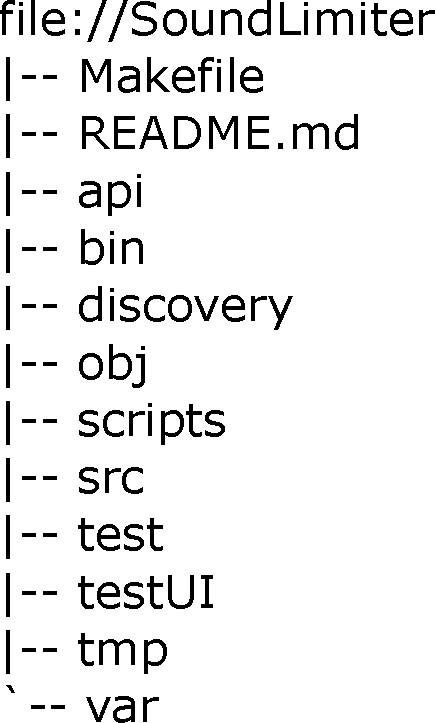
\includegraphics[width=.45\textwidth]{figuras/lms11-files.pdf}
	    \caption[Estructura de directorios del proyecto]{Estructura de directorios del proyecto. Los dos primeros elementos son ficheros, no directorios}
	    \label{fig:lms11-files}
    \end{minipage}
    \hfill
    \begin{minipage}{.45\textwidth}
        \centering
        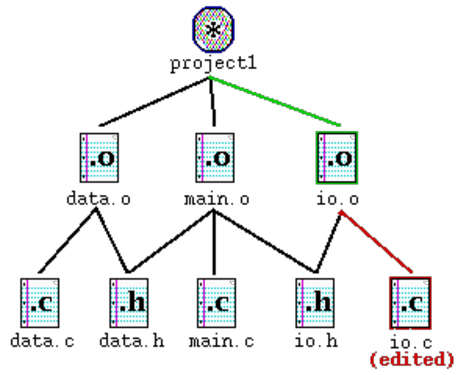
\includegraphics[width=1\textwidth]{figuras/make.pdf}
        \caption[Compilación con Make]{Compilación con Make. Sólo se recompila el fichero modificado.}
        \label{fig:make}
    \end{minipage}
\end{figure}

\clearpage

\begin{lstlisting}[language=make, caption={Makefile del LM11}, label={lst:lms11-make}]
###############################################################################
#
# Limitador de Sonido - \glsname{granasat}
# Grado en Ingeniería Informática
#
# 2021 - Alejandro Ruiz Becerra <alexruiz@correo.ugr.es>
# ---------------------------------------------
#
# Fichero Makefile para generación de ejecutables
#
###############################################################################

SLR_DIR = ~/SoundLimiter

# -------------------------------------
# Compilador (C++)
# -------------------------------------
CXX = g++

# -------------------------------------
# Banderas para el compilador (C++)
# -------------------------------------
CXXFLAGS = -std=c++17 -g -O3 -I$(shell pwd)
CXXEXTRA = -Wno-write-strings -Wno-unused-result -mcpu=arm7

# ---------------------------------------------
# Macros generales
# ---------------------------------------------
# Definición de directorios principales
# ---------------------------------------------
SRC_DIR := ./src
BIN_DIR := ./bin
OBJ_DIR := ./obj
TEST_DIR := ./test

# ----------------------- ########## ----------------------- #
#                      OBJETIVOS GENERALES
# ----------------------- ########## ----------------------- #
all: $(BIN_DIR)/analyzer	     \
	 $(BIN_DIR)/calibrator       \
	 $(BIN_DIR)/get-config	     \
	 $(BIN_DIR)/get-data         \
	 $(BIN_DIR)/get-status	     \
	 $(BIN_DIR)/init-station     \
	 $(BIN_DIR)/sound-limiter    \
	 $(BIN_DIR)/sound-register   \
	 $(BIN_DIR)/update-config    \
	 $(BIN_DIR)/hardware-controller

clean:
	rm -rf $(OBJ_DIR)

superclean: clean
	rm -rf $(BIN_DIR)

... OBJETIVOS
\end{lstlisting}

\subsection{Re-utilización de código}

El objetivo es importar aquellos módulos seleccionados de los LM durante la etapa de \nameref{cap:capitulo4} al nuevo limitador, con el objetivo de \commillas{echarlos a andar} sobre el nuevo hardware. Mediante el uso de los diagramas de clases y de dependencias generados durante el proceso de ingeniería inversa, se ha podido extraer el código estrictamente necesario para compilar los programas seleccionados de forma independiente. Antes de llevarlos al nuevo limitador se han sometido a un proceso de refactoring en el que se ha intentado solucionar los problemas vistos en la sección \ref{sec:errores}.

Algunos de los ficheros han sido renombrados por nombres más descriptivos y para evitar confusiones. Por ejemplo cada uno de los módulos disponía de un fichero \texttt{main.cpp} en el que se encuentra el punto de entrada al programa. En la nueva estructura todos los ficheros de código fuente se encuentran al mismo nivel y no se pueden tener varios ficheros con el mismo nombre, además de ser poco descriptivo. En su lugar se han renombrado estos ficheros por \texttt{<Programa>Main.cpp} para distinguir a cada uno de ellos (por ejemplo \texttt{RegistradorMain.cpp}).

Un caso más importante es el del registrador, en el que tanto la clase que implementa el registrador (\texttt{Registrador.cc} en \acrshort{LM9}), como el fichero que contiene el programa principal (\texttt{Registrador.cpp} en \acrshort{LM9}) no sólo compartían el mismo nombre, sino que definen e implementan la funcionalidad en el mismo fichero (no separan en \texttt{.h} y \texttt{.cpp}).

En el nuevo software, se ha divido las definiciones de las clases de su implementación y se ha separada la funcionalidad del registrador de su función principal, ampliando el número de ficheros de 2 a 5, pero bien estructurados, formateados y comentados. Además de todo esto, la salida del programa se ha actualizado para hacer uso del framework \textbf{nCurses} en lugar de la salida estándar, de forma que la vista se actualiza en lugar de sumarse a la salida anterior, lo que hacía que la salida del programa fuera poco legible. \\
Estos ficheros reciben el nombre de \texttt{GestorRegistro} (\texttt{.hpp} y \texttt{.cpp}), \texttt{Registrador} (\texttt{.hpp} y \texttt{.cpp}) y \texttt{RegistradorMain.cpp}

\subsection{Novedades}

Aunque es cierto que el grueso de la implementación del sistema ha sido heredada, también ha sido necesaria la implementación de clases y programas

Las novedades en el diseño se traducen en la implementación de nuevas clases y programas, descritos en la sección de \nameref{cap:capitulo5}.

Principalmente todo lo relacionado con el nuevo hardware ha necesitado una nueva implementación, por razones obvias. La comunicación con el hardware se ha realizado mediante las librerías \textbf{WiringPi}, \textbf{I2C} y \textbf{WiringSPI}. Los compañeros de \glsname{granasat}, \myMateLuis\ y Sharif Al-Husein Raie, con mucha más experiencia que yo en el campo de la electrónica y sistemas embebidos, me han proporcionado programas de prueba que implementan la comunicación con los componentes hardware del equipo. Estos programa han sido de gran ayuda ya que han supuesto una base y una guía importante a seguir, tanto que a veces tan solo ha sido necesario encapsular el código en clases e integrarlo en el proyecto.\\
\acrshort{PGA}, \acrshort{LCD}, \acrshort{LED}s, buzzer y la detección de micrófono hacen uso de estas librerías.

En las versiones estudiadas, el configurador formaba parte del programa \texttt{utilslr}. En el nuestro software se ha implementado un programa llamado \texttt{update-config} cuya única responsabilidad es actualizar la configuración del sistema a partir del contenido del fichero \texttt{tmp.conf}.

\subsubsection{La API-REST}

Sin duda el cambio la introducción de una \glsname{API-REST} al sistema para consultar su estado y controlarlo de forma externa supone la novedad más rompedora a nivel de software. La antigua aplicación, aunque funcional y bien desarrollada visualmente, tenía problemas importantes que han hecho imposible tu portabilidad. La \glsname{API-REST} se ha diseñado precisamente bajo este pretexto y con el fin de solucionar el problema expuesto.

La \glsname{API-REST} ha sido implementada en \textbf{\textit{Python}}, concretamente mediante el uso del framework de \textbf{\textit{Connexion}}, construido sobre el framework de \textit{Flask} y diseñado para funcionar mano a mano con \textbf{\textit{Swagger/OpenAPI}} \cite{swagger}. Gracias a la maravillosa herramienta de OpenAPI \cite{openapi} se ha podido generar código de forma automática tan sólo instalando un contenedor de Docker. La herramienta permite generar código en una gran variedad de lenguajes y marcos de trabajo, gracias a los patrones que estos frameworks definen, y todo esto tomando como origen el fichero de definición de la \glsname{API-REST}, un fichero en formato YML o \acrshort{JSON} en el que se definen los servicios que expone la \glsname{API-REST}, así como los modelos y controladores que necesita.

La definición de la \glsname{API-REST} del sistema se extiende casi a las 1 000 líneas de código YML. \\

\begin{lstlisting}[language=python, caption={\glsname{API-REST} del LM11}, label={lst:lms11-api-conf}]
def update_config(configurable_properties: ConfigurableProperties = None):
    """Updates limiter's configuration

    Updates limiter's configuration based on the data
    received within this POST request. The data must be on
    JSON format.

    See the example below for a list of all available
    properties that are configurable.

    :param configurable_properties: List of every configurable
           property of the sound limiter. None of the fields are required.
    :type configurable_properties: dict | bytes

    :rtype: GenericResponse
    """
    if connexion.request.is_json:
        configurable_properties = ConfigurableProperties.from_dict(connexion.request.get_json())

        # Construir conf.tmp con los datos recibidos desde el JSON
        configurator = Configurator(configurable_properties)
        print(configurable_properties)
        configurator.configure()

        # Una vez exportados los datos al fichero conf.tmp, lanzar el configurador.
        cmd = "/root/SoundLimiter/bin/update-config"

        try:
            success = os.popen(cmd)
            if success:
                status_code, message = 200, "Configuration updated"
            else:
                status_code, message = 500, "An unexpected error occured during the configuration"
            return GenericResponse(status_code, message)
        except OSError:
            return GenericResponse(503, "Could not query limiter's configurator service")
\end{lstlisting}

\section{Resultados}

AÑADIR IMÁGENES DE API EN LIMITADOR
